\section{无限维闭球不紧}
\label{sec:fvec-closed-ball-noncompact}

在$\mathbb R^d$中，有界序列总有收敛子列，闭有界集上的连续函数总取到最小值。许多存在性论证都是这样进行的：先找一列越来越好的近似，再从中抽出收敛子列，最后说明极限就是所求的对象。本节说明，这条路在无限维空间中会断。

标准单位列已经显示了问题所在。在$c_0$中用各项之差的上确界作距离，$e_m$与$e_n$（$m\neq n$）在第$m$项相差$1$，其余各项相差不超过$1$，所以二者的距离恰为$1$。这些点都在以零数列为中心、半径为$1$的闭球里，它们彼此隔开，没有任何子列收敛。

本节要证明这不是$c_0$的特殊现象，而是所有无限维赋范空间的共同性质。这里需要用距离衡量“彼此隔开”，所以先回顾卷二的范数。线性空间$V$上的范数$\lVert\cdot\rVert$是满足正定性、齐次性$\lVert cx\rVert=\lvert c\rvert\lVert x\rVert$与三角不等式的非负函数，它诱导距离$d(x,y)=\lVert x-y\rVert$；配有范数的空间称为赋范空间。

有限维情形的范数理论可参考\BookChapterRef{chap:normed-spaces}{卷二第3章“赋范空间”}，无限维的系统讨论在第~\ref{chap:function-normed-spaces}章。本节只用这些公理和距离的语言。

\paragraph{有限维子空间是闭集}
下面的构造要用到这样一个事实：在任意赋范空间中，有限维子空间是闭集。平面上过原点的直线、三维空间中过原点的平面都是闭集，无限维的环境空间里这一点仍然成立。

\begin{lemma}[有限维子空间闭性]
\label{lem:fvec-finite-subspace-closed}
设$X$是赋范空间，$Y\subseteq X$是有限维线性子空间。则$Y$是$X$中的闭集。
\end{lemma}

\begin{proof}
设$y_n\in Y$且在$X$中$y_n\to x$，要证$x\in Y$。收敛序列是柯西列，所以$\{y_n\}$是$Y$中的柯西列。

把$X$的范数限制在$Y$上，$Y$成为一个有限维赋范空间。卷二证明了有限维赋范空间在任意范数下都完备，所以$\{y_n\}$在$Y$中收敛到某个$y$。

这个$y$也是$\{y_n\}$在$X$中的极限。第~\ref{chap:metric-spaces}章说明度量空间中的极限唯一，所以$x=y\in Y$。
\end{proof}

这个论证没有要求$X$完备，只用到$Y$自身的完备性。由闭性，若$x_0\notin Y$，则$x_0$到$Y$的距离
\[
 d(x_0,Y)=\inf_{y\in Y}\lVert x_0-y\rVert
\]
严格为正：否则可在$Y$中取一列$y_n$使$\lVert x_0-y_n\rVert\to0$，闭性给出$x_0\in Y$，矛盾。

\paragraph{Riesz引理}
要在无限维空间中造出彼此远离的单位向量，先看$\mathbb R^2$中是怎样做的。取一条过原点的直线$Y$和线外一点$x_0$，从$x_0$向$Y$作垂线，垂足是$Y$上离$x_0$最近的点。$x_0$减去垂足再归一化，就得到与$Y$垂直的单位向量，它到$Y$的距离恰为$1$。

一般赋范空间没有垂直，$Y$上的最近点也可能不存在，所以要退一步：不取最近点，而取一个几乎最近的点$y_0$。图~\ref{fig:fvec-riesz-lemma}画出了这个做法。$x_0-y_0$不再与$Y$垂直，归一化后的向量$x$略微倾斜，但它到$Y$的距离仍接近$1$。

\begin{BookInlineFigure}
  \centering
  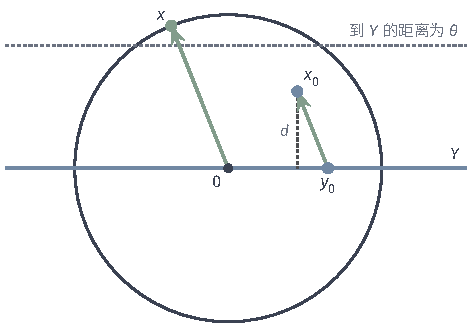
\includegraphics[width=79.904mm]{figures/04-spaces-measures-and-geometry/03-function-spaces/tikz/fvec-riesz-lemma/figure.pdf}
  \caption{Riesz引理的构造在$\mathbb R^2$中的样子。蓝色直线是子空间$Y$，圆是单位球面。$x_0$到$Y$的距离为$d$，$y_0$是$Y$上一个几乎最近的点。把向量$x_0-y_0$（绿色）平移到原点并归一化，得到单位向量$x$，它落在虚线上方，到$Y$的距离不小于$\theta$。}
  \label{fig:fvec-riesz-lemma}
\end{BookInlineFigure}

把这个几何过程写成不等式，就得到下面的引理。

\begin{lemma}[Riesz引理]
\label{lem:fvec-riesz}
设$X$是赋范空间，$Y\subsetneq X$是闭线性子空间，$0<\theta<1$。则存在$x\in X$，使$\lVert x\rVert=1$，并且
\begin{equation}
 \lVert x-y\rVert\geq\theta,\qquad y\in Y.
 \label{eq:fvec-riesz}
\end{equation}
\end{lemma}

\begin{proof}
取$x_0\in X\setminus Y$，记$d=d(x_0,Y)$。由$Y$闭，$d>0$。因为$d/\theta>d$，由下确界的定义可以取$y_0\in Y$使
\[
 d\leq\lVert x_0-y_0\rVert\leq\frac{d}{\theta}.
\]
令$c=\lVert x_0-y_0\rVert$，并取$x=(x_0-y_0)/c$，则$\lVert x\rVert=1$。

对任意$y\in Y$，把$x-y$通分，写成
\[
 x-y=\frac{x_0-(y_0+cy)}{c}.
\]
括号里的$y_0+cy$仍属于线性子空间$Y$，所以分子的范数至少是$d$。于是
\[
 \lVert x-y\rVert\geq\frac{d}{c}\geq\frac{d}{d/\theta}=\theta.
\]
\end{proof}

引理的两个条件都不能去掉。先看“$Y$闭”。在$c_0$中取$Y=c_{00}$，它是真子空间，但不闭。对任意$x\in c_0$，截断$s_N$属于$Y$，并且
\[
 \sup_{k\geq1}\lvert x_k-(s_N)_k\rvert=\sup_{k>N}\lvert x_k\rvert\to0,
\]
所以每个$x$到$Y$的距离都是$0$，式~\eqref{eq:fvec-riesz}对任何$\theta>0$都不成立。

再看$\theta<1$。在有限维中$\theta=1$可以取到，因为最近点存在；无限维中最近点可能取不到，$\theta=1$就可能失败。下面是一个能手算的例子。

\begin{example}[$\theta=1$可能失败]
\label{ex:fvec-riesz-theta-one}
令$X=\{f\in C[0,1]:f(0)=0\}$，范数取$\lVert f\rVert=\max_t\lvert f(t)\rvert$，令
\[
 Y=\Bigl\{f\in X:\int_0^1f(t)\,dt=0\Bigr\}.
\]
$Y$是闭子空间，因为$\lvert\int f-\int g\rvert\leq\lVert f-g\rVert$，积分为零的性质在一致极限下保持。

任取$X$中的单位向量$x$，构造$Y$中逼近它的元素。令$h_n(t)=\min(nt,1)$，则$h_n\in X$，$\lVert h_n\rVert=1$，并且积分为
\[
 \int_0^1h_n(t)\,dt=1-\frac1{2n}.
\]
记$I=\int_0^1x(t)\,dt$，令
\[
 y_n=x-\frac{I}{1-\frac1{2n}}h_n,
\]
它的积分为$I-I=0$，所以$y_n\in Y$。

$x$到$y_n$的距离由$h_n$的系数给出：
\[
 \lVert x-y_n\rVert=\frac{\lvert I\rvert}{1-\frac1{2n}}.
\]
令$n\to\infty$，得到$d(x,Y)\leq\lvert I\rvert$。而$x$连续且$x(0)=0$，所以在$0$附近$\lvert x\rvert<\tfrac12$，又处处有$\lvert x\rvert\leq1$，于是$\lvert I\rvert<1$。

所以$X$中每个单位向量到$Y$的距离都严格小于$1$，$\theta=1$的结论不成立。
\end{example}

\paragraph{两两远离的单位向量}
现在设$X$是无限维赋范空间，用Riesz引理逐个构造单位向量。任取一个单位向量$e_1$。设已经得到单位向量$e_1,\ldots,e_n$，令
\[
 Y_n=\operatorname{span}\{e_1,\ldots,e_n\}.
\]
$Y_n$是有限维子空间，由引理~\ref{lem:fvec-finite-subspace-closed}是闭集；$X$无限维，所以$Y_n\neq X$。对$Y_n$与$\theta=\tfrac12$应用引理~\ref{lem:fvec-riesz}，得到单位向量$e_{n+1}$，它到$Y_n$中每一点的距离都至少为$\tfrac12$。

这样得到的序列$\{e_n\}$有两条性质。其一，它线性无关：$e_{n+1}$到$Y_n$的距离为正，所以$e_{n+1}\notin Y_n$，每个新元素都不能由之前的元素线性表示。其二，它两两远离：对$m<n$，$e_m\in Y_{n-1}$，所以
\begin{equation}
 \lVert e_n-e_m\rVert\geq\frac12,\qquad m\neq n.
 \label{eq:fvec-separated-sequence}
\end{equation}
第~\ref{chap:function-normed-spaces}章构造不等价范数时，还会用到这里的单位列$\{e_n\}$。

有了这列向量，闭球不紧的结论就只差一步。

\begin{theorem}[无限维闭球不紧]
\label{thm:fvec-closed-ball-noncompact}
设$X$是无限维赋范空间。则闭单位球$\bar B=\{x\in X:\lVert x\rVert\leq1\}$不是全有界的，从而不紧。更一般地，对任意$a\in X$与$r>0$，闭球$\{x:\lVert x-a\rVert\leq r\}$都不紧。
\end{theorem}

\begin{proof}
全有界要求对每个$\varepsilon>0$，$\bar B$都能被有限个半径为$\varepsilon$的开球覆盖。取$\varepsilon=\tfrac14$。半径$\tfrac14$的开球中任意两点的距离小于$\tfrac12$，由式~\eqref{eq:fvec-separated-sequence}，每个这样的球至多含有一个$e_n$。$\bar B$中有无穷多个$e_n$，有限个球盖不住它们，所以$\bar B$不全有界。第~\ref{chap:metric-spaces}章证明了紧度量空间必定全有界，故$\bar B$不紧。

也可以直接从序列看：$\{e_n\}$的任何子列都满足式~\eqref{eq:fvec-separated-sequence}，不是柯西列，因而不收敛。

对一般的闭球，映射$x\mapsto a+rx$把$\bar B$一一地映成该闭球，并把距离乘以$r$。若该闭球紧，则$a+re_n$有收敛子列，相应的$e_n$子列也收敛，矛盾。
\end{proof}

证明从头到尾没有用到$X$的完备性。不紧的原因不是“缺少极限点”，而是有界的区域里装得下无穷多个互相隔开的点。

有限维中这样的点只能有有限个，用体积就能数出来。设$\mathbb R^d$的单位球中有$N$个点两两距离至少为$\tfrac12$。以这些点为中心、半径$\tfrac14$的开球两两不交，并且都含在半径$\tfrac54$的球内。比较体积，得到
\[
 N\Bigl(\frac14\Bigr)^d\leq\Bigl(\frac54\Bigr)^d.
\]
约去公因子，就是
\begin{equation}
 N\leq5^d.
 \label{eq:fvec-packing-bound}
\end{equation}
所以$\mathbb R^2$的单位圆盘中至多有$25$个这样的点。这个上界随$d$增大而迅速增大，$d$无限时不再有任何上界，这就是无限维中闭球不紧的直观原因。图~\ref{fig:fvec-bounded-noncompact}(a)是$d=2$的情形。

\paragraph{连续函数的例子}
Riesz引理给出的是存在性。在具体的函数空间中，往往可以直接写出没有收敛子列的有界序列。考虑$C[0,1]$，以两个函数之差的最大绝对值
\[
 d(f,g)=\max_{x\in[0,1]}\lvert f(x)-g(x)\rvert
\]
为距离。连续函数在闭区间上取到最大值，所以$d$有定义；它来自范数$\max_x\lvert f(x)\rvert$，按这一距离收敛就是一致收敛。

\begin{BookInlineFigure}
  \centering
  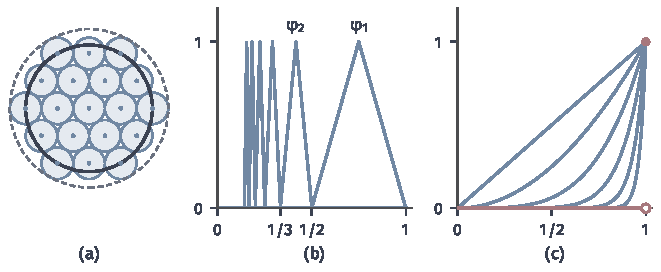
\includegraphics[width=112mm]{figures/04-spaces-measures-and-geometry/03-function-spaces/matplotlib/fvec-bounded-noncompact/figure.pdf}
  \caption{有界而不紧。(a)$\mathbb R^2$单位圆盘（实线）内的$19$个点，两两距离不小于$\tfrac12$，半径$\tfrac14$的小圆盘互不重叠，全部落在半径$\tfrac54$的虚线圆内。(b)在$C[0,1]$中，前六个鼓包$\varphi_n$的支撑互不重叠，高度都是$1$。(c)蓝色为$x^n$（$n=1,2,4,8,16,32$），红色为逐点极限：$[0,1)$上为$0$，在$1$处取$1$。}
  \label{fig:fvec-bounded-noncompact}
\end{BookInlineFigure}

最接近标准单位列的是一列鼓包。对$n\geq1$，令$\varphi_n$在区间$[\tfrac1{n+1},\tfrac1n]$的中点取$1$，在区间两端取$0$，在区间上线性插值，在区间外恒为$0$。图~\ref{fig:fvec-bounded-noncompact}(b)显示，这些鼓包各占一段位置，相当于各占一个“坐标”。

当$m\neq n$时，$\varphi_m$与$\varphi_n$的支撑至多在一点相接，而两函数在该点都为零，所以每点至多有一个函数非零。在$\varphi_n$的峰值点，差的绝对值为$1$，于是
\[
 d(\varphi_m,\varphi_n)=1,\qquad m\neq n.
\]
它们都在以零函数为中心、半径为$1$的闭球内，没有任何子列收敛。

再看$f_n(x)=x^n$，它的表现不同。每个$f_n$满足$0\leq x^n\leq1$，所以也都在同一个闭球内。相邻两项的差$x^n(1-x)$在$x=\tfrac n{n+1}$处取最大值，由此
\[
 d(f_n,f_{n+1})=\Bigl(\frac n{n+1}\Bigr)^n\frac1{n+1}\leq\frac1{n+1},
\]
相邻两项越来越近。序列看上去在收敛，但它仍然没有任何按$d$收敛的子列。

设子列$f_{n_k}$按$d$收敛到某个$g\in C[0,1]$。一致收敛推出逐点收敛，所以对每个$x$，$g(x)=\lim_kx^{n_k}$。当$0\leq x<1$时这个极限是$0$，当$x=1$时是$1$。于是$g$在$[0,1)$上恒为$0$而$g(1)=1$，在$1$处不连续，与$g\in C[0,1]$矛盾。

两个例子失败的方式不同。鼓包的逐点极限是零函数，它就在$C[0,1]$中，可是每个鼓包离它的距离总是$1$，逐点接近不等于一致接近。$x^n$的逐点极限跑出了$C[0,1]$，候选极限根本不在空间里。函数类在什么附加条件下恢复紧性，例如要求一致有界并且等度连续，是第~\ref{chap:metric-space-maps}章和第~\ref{chap:function-class-covers}章的内容。
